\label{section:results-and-discussion}
%
\begin{figure}[t]
    \centering
    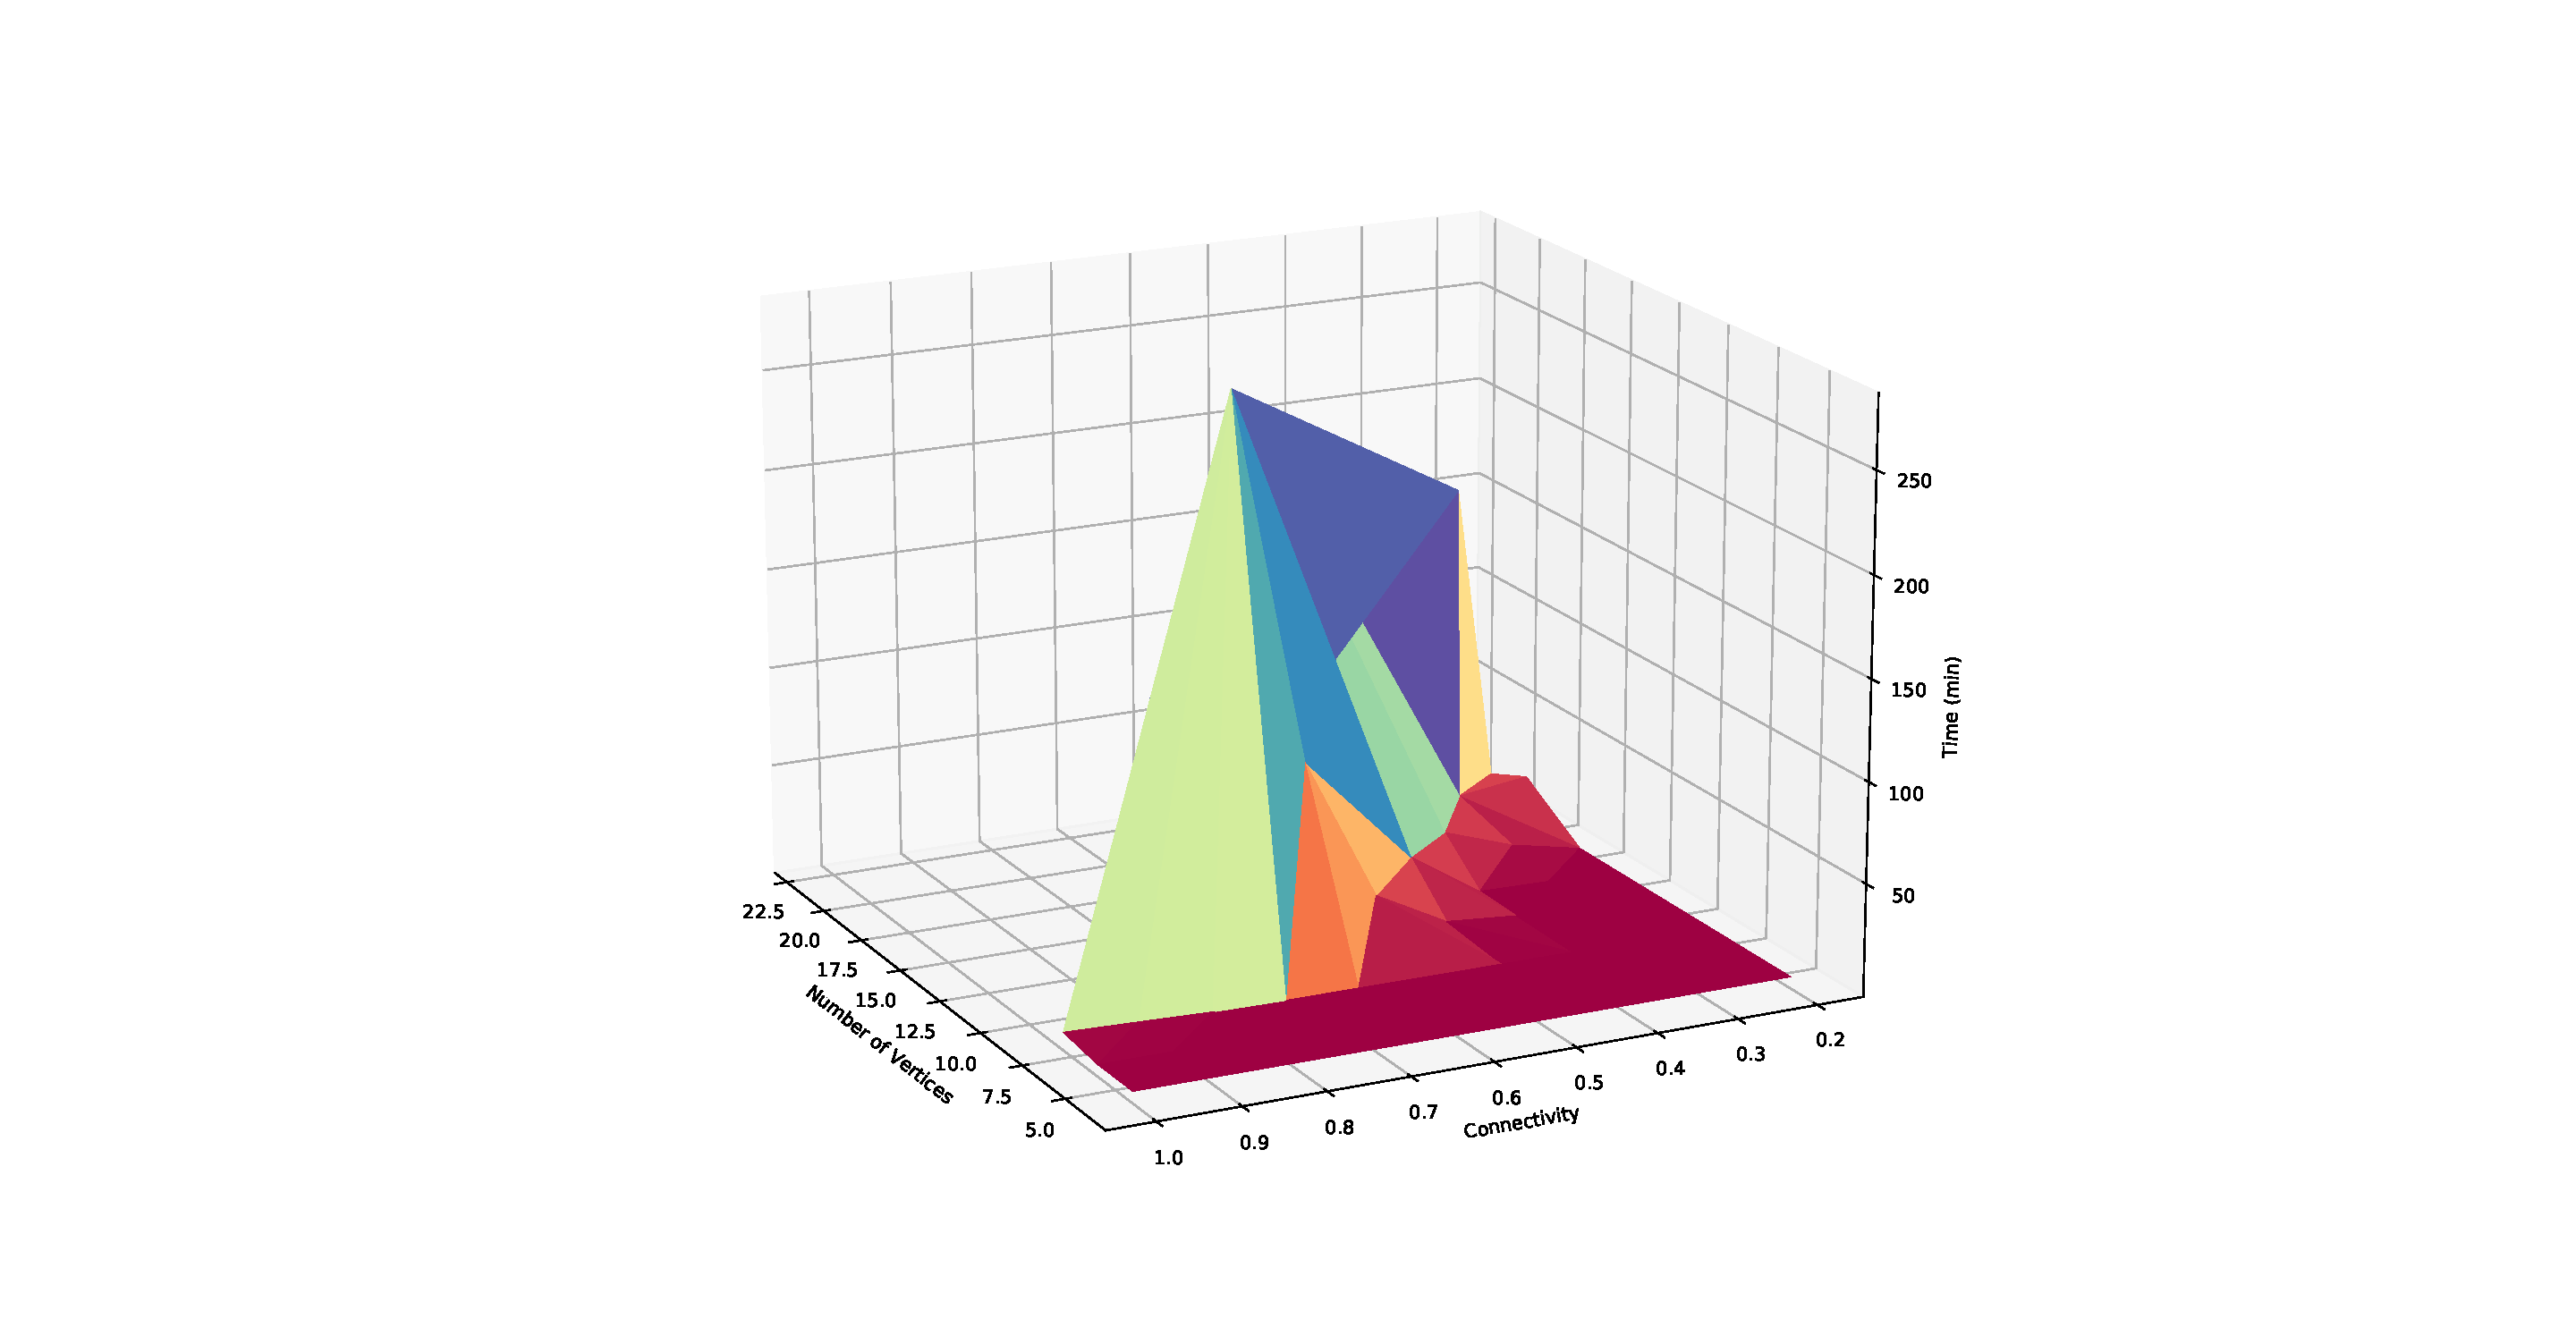
\includegraphics[width=1\linewidth]{Figures/big_ol_cliff.pdf}
    \caption{Results of the \ac{smt} encoding on randomly generated
      Erd\H{o}s-R\'{e}nyi graphs. The z-axis is runtime in minutes, with
      connectivity on the y-axis and vertex count on the x-axis. We see that
      runtime explodes at an interaction point between vertex count and
      connectivity.}%
    \label{fig:results}
\end{figure}%

\autoref{fig:results} displays the runtime of the prototype \ac{smt} method to
find a minimum feedback arc set for randomly generated Erd\H{o}s-R\'{e}nyi
graphs. We observe that as the number of vertices increases the runtime
exponentially increases, for example with x = 5 vertices the runtime is stable,
however at x = 12 the runtime becomes greater than 2 hours (clock time).
Similarly, highly connected graphs the runtime exponentially increases. Consider
the difference between 20\% connectivity and 70\% connectivity, at 20\% we see
the runtime stay low as vertex count increases, however at 70\% connectivity the
runtime quickly grows to the order of hours for a graph with just 10 vertices.
Lastly, we observe an interaction between the vertex count and connectivity
parameters which creates a runtime barrier.

Our observations are not entirely unexpected. Since our method is centered
around a cycle matrix the number of cycles in the graph should impact the
runtime of the solver. What is unexpected in our study is the magnitude of the
runtime performance. Industrial strength \ac{sat} and \ac{smt} solvers are used
to solve constraints with millions of variables and several million
clauses~\cite{10.5555/1550723}, yet our results here indicate a ludicrously
difficult problem for the \ac{smt} solver to solve.

We speculate on possible causes. First, it could be that our prototype is
translating the constraints to its internal z3 instance poorly, leading to a
high degree of garbage collection pressure in the python runtime. Second, our
encoding could accidentally be creating \ac{smt} problems that are in the
\emph{phase change}~\cite{Gent94thesat} region of the \ac{smt} solver.

The phase change of \ac{sat} and \ac{smt} solvers is the region where difficult
to solve problems occur. The phase change is characterized by the ratio of
clauses to variables. Conceptually if we have many clauses but not many
variables then we are over-constrained and thus it is easy to find \rn{unsat}.
However, if we have many variables and not many clauses then we are
under-constrained and it is easy to find \rn{sat}. The difficult region for a
\ac{sat} or \ac{smt} solver occurs when the number of clauses and variables are
balanced. Thus, it could be the case that our encoding creates \ac{smt} problems
in this range. Similarly, it could be that our encoding as a simple summation
over symbolic variables is naive. A more efficient implementation would use high
performance \ac{smt} structures such as \rn{Bit-Vectors}~\cite{BarFT-SMTLIB}
which have been successfully used to solve constraint networks in electronic
design\cite{10.5555/1550723}.


Third, there might be specific features of graphs which lead to
easier or more difficult \ac{smt} problems. For example, previous research has
found that tournament graphs, such as \autoref{fig:tournament-graph} are easier
to solve than the general case.

%%% Local Variables:
%%% mode: latex
%%% TeX-master: "../main"
%%% End: